\chapter{Approach and Implementation}
\label{ch:approach}
In this chapter the basic work flow is described in detail. The process is mainly driven by an exploratory approach, but follows primarily Farines and Whiteheads~\cite{farine2015constructing} primary steps and key considerations for social network analysis to non-human animal data. The adapted and resulting process is visualized in figure~\ref{fig:process}.

The dataset was first analysed regarding data quality and to form an understanding of the dataset and the behaviour of bees in general. Those findings were used to define nodes and infer associations to build the network, respectively derive the parameters for the network pipeline. The static and temporal networks are analysed using network science tools and methods. For testing hypothesis the networks are combined with spatial and age information. Each step is explained within the following sections.

\begin{figure}[htb]
	\centering
	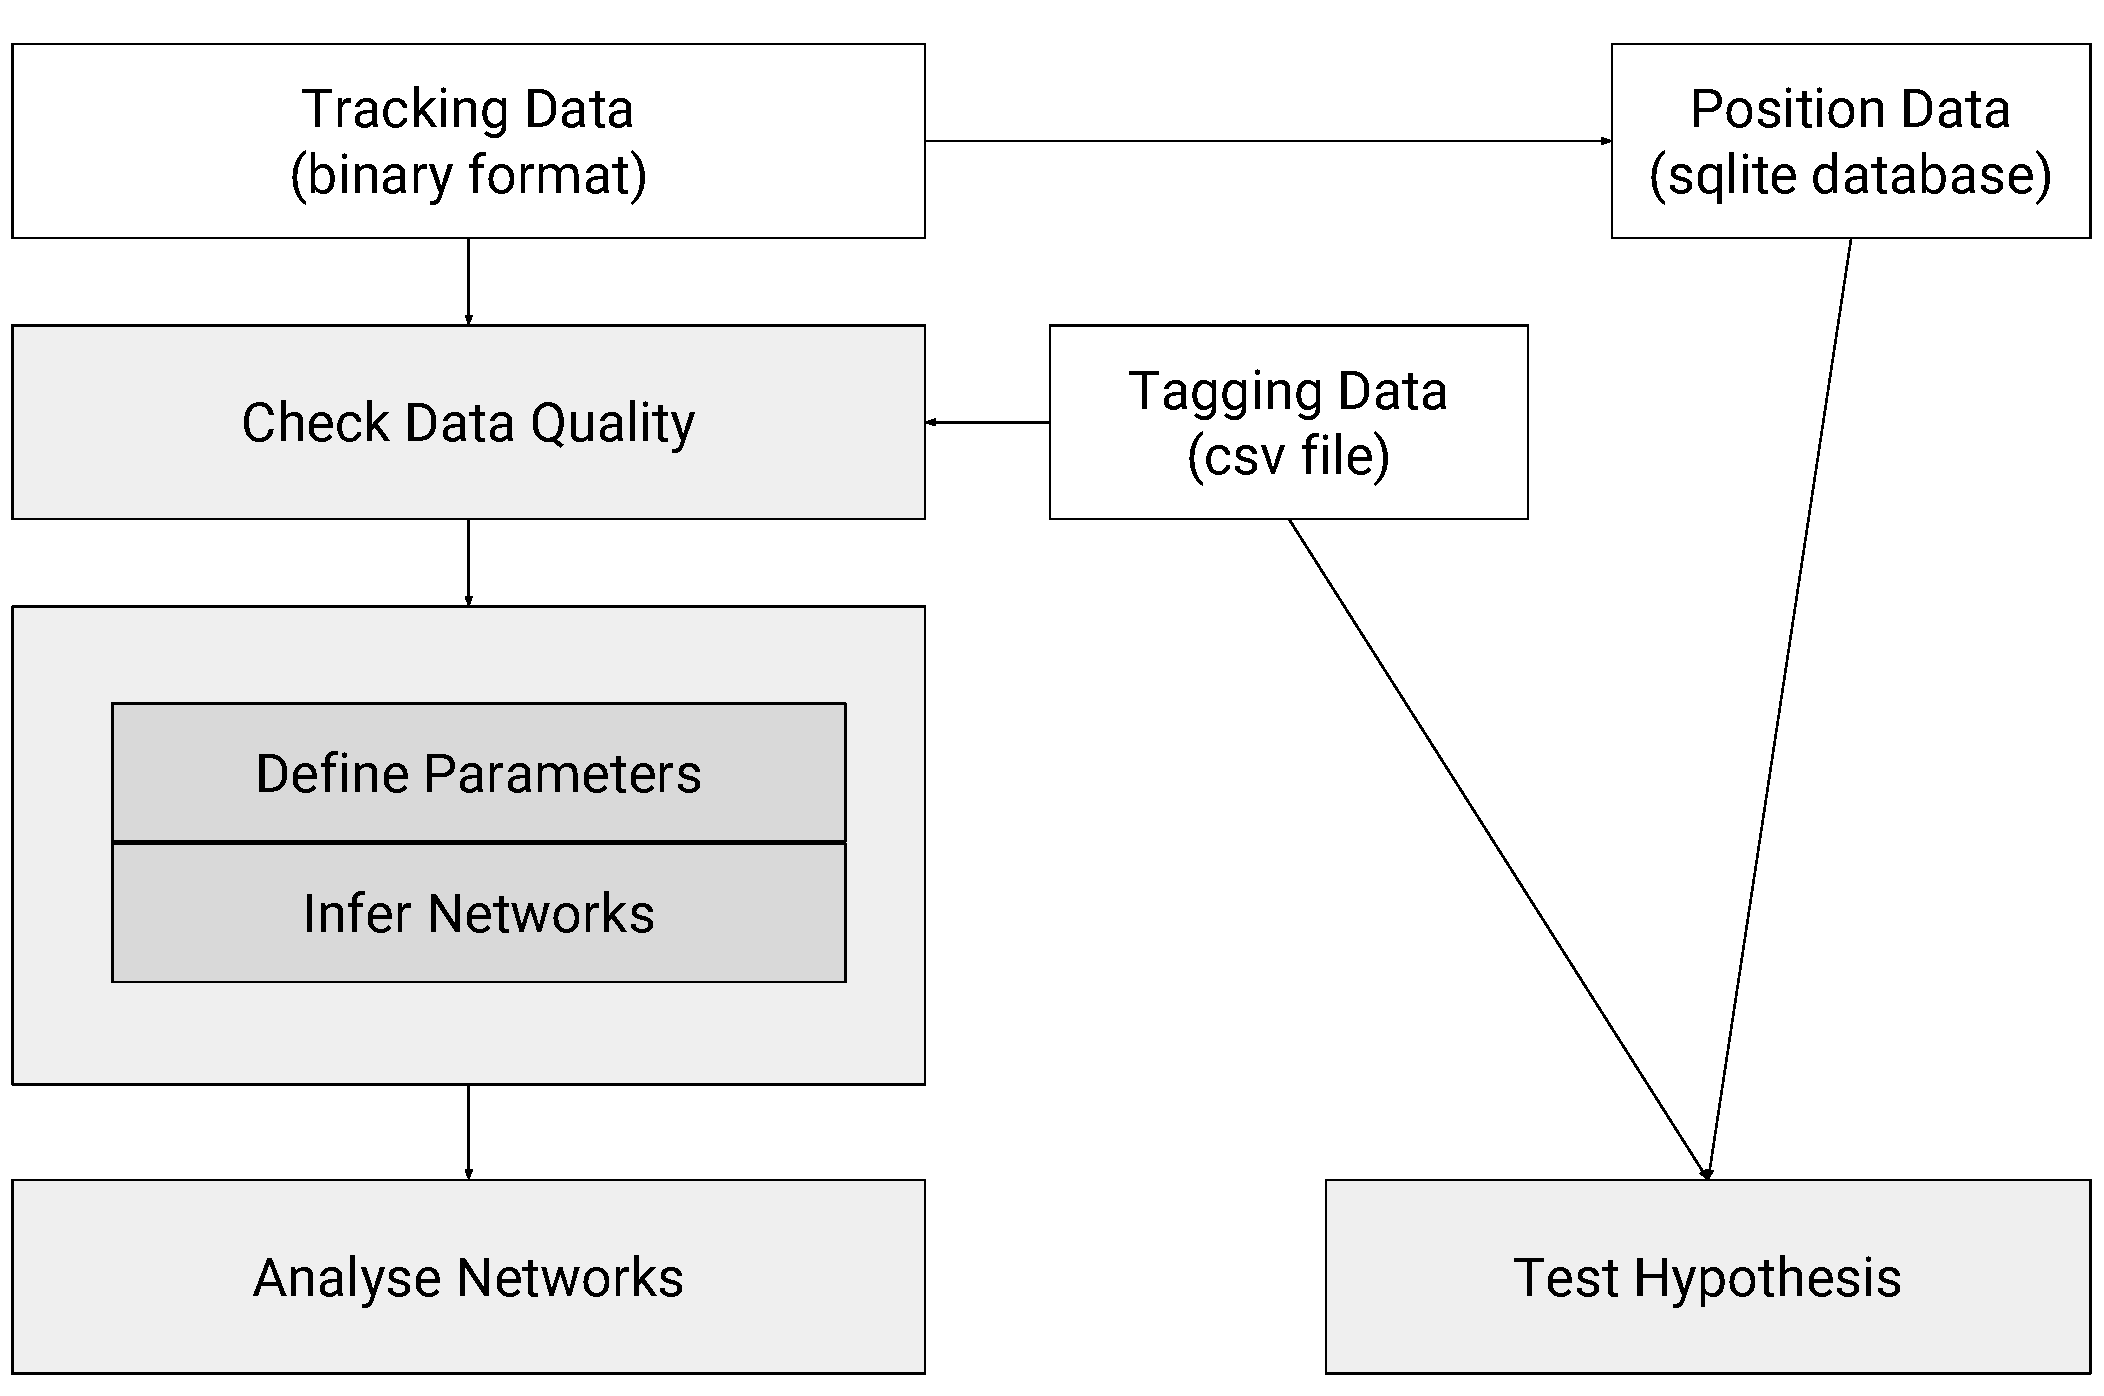
\includegraphics[width=0.8\textwidth]{Figures/process}
	\caption{Steps of the Research Approach}
	\label{fig:process}
\end{figure}

\begin{figure}[htb]
	\centering
	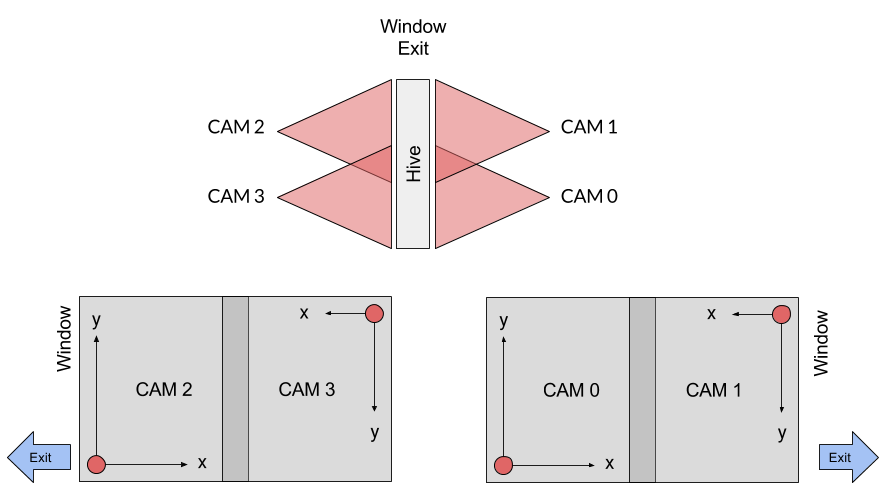
\includegraphics[width=0.5\textwidth]{Figures/setupCams}
	\caption[Camera Setup in 2016]{Camera Setup in 2016}
	\label{fig:cams}
\end{figure}


\section{The Dataset}
\label{sec:dataset}
The dataset derives from video files, that capture tagged honey bees of one colony in an observation hive.
Each individual of the colony, including about 3000 bees, were tagged with circular 12-bit markers (figure~\ref{fig:markers}, section~\ref{ch:intro}). Four cameras were used to film the hive. The setup of the cameras is illustrated in figure~\ref{fig:cams}.

\begin{figure}[htb]
	\centering
	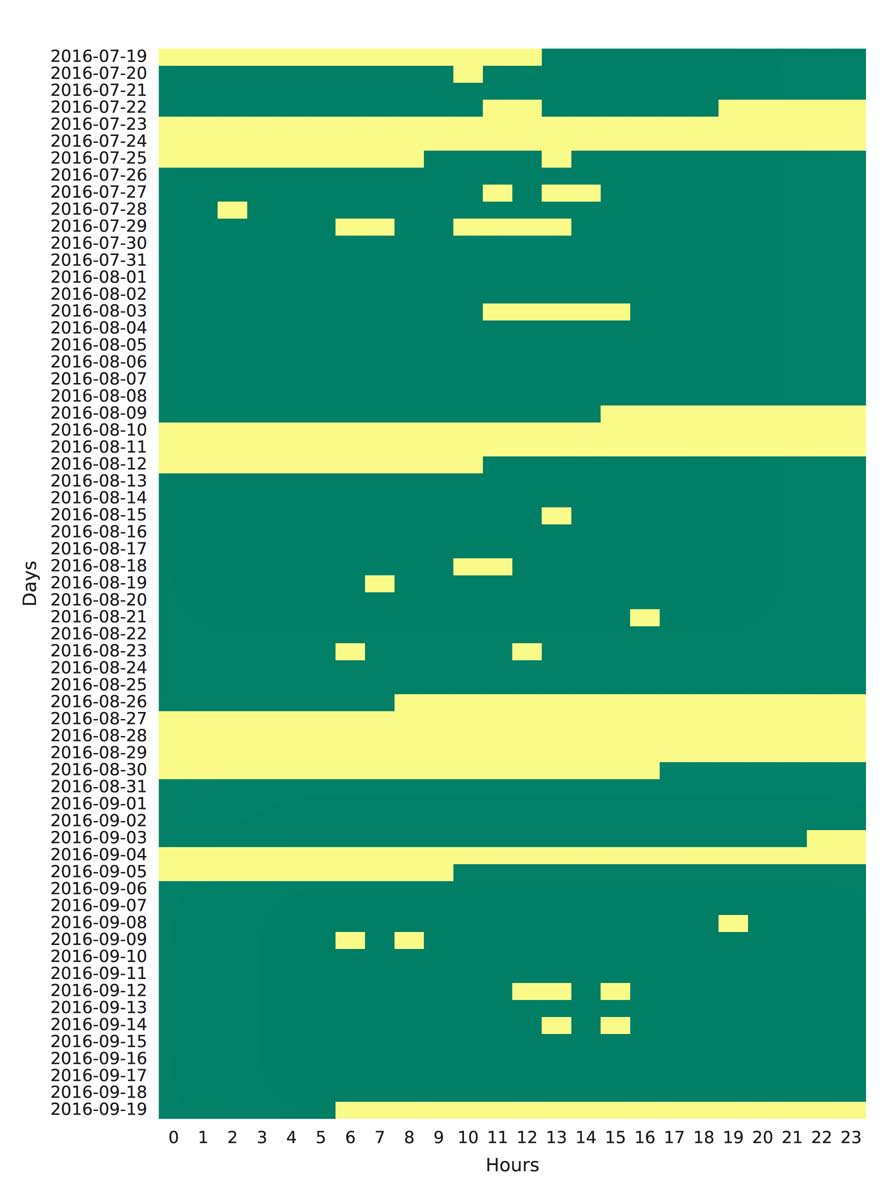
\includegraphics[width=0.4\textwidth]{Figures/recording}
	\caption[Recording Season]{Recording Season with maintainance and failures: \emph{Green} indicates recording went without any big interruption; \emph{Yellow} indicates maintainance work or technical failures of one or all cameras. This is calculated using the expected number of files produced by each camera per hour.}
	\label{fig:period}
\end{figure}

\begin{figure}[htb]
	\centering
	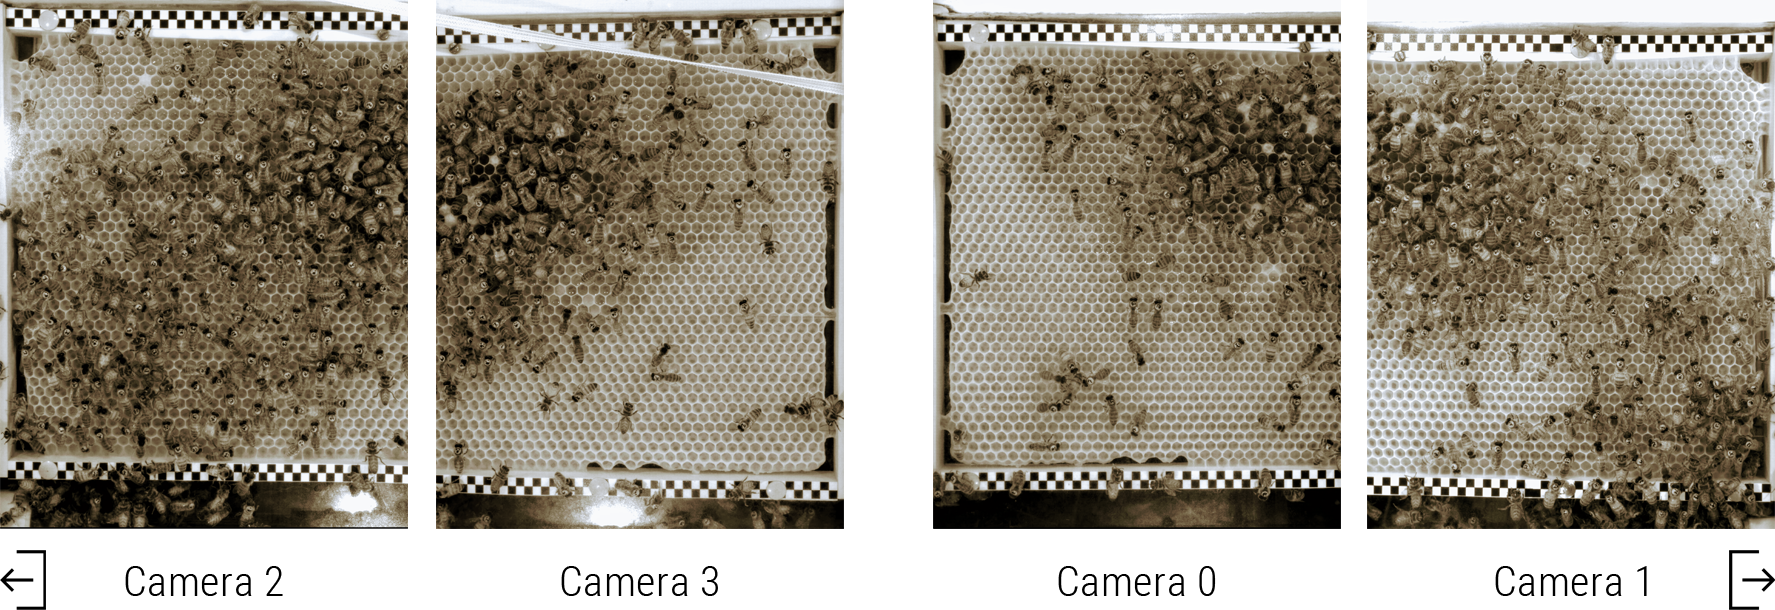
\includegraphics[width=0.8\textwidth]{Figures/beesClose}
	\caption[xxx]{xxx}
	\label{fig:veryclose}
\end{figure}


\begin{figure}[htb]
	\centering
	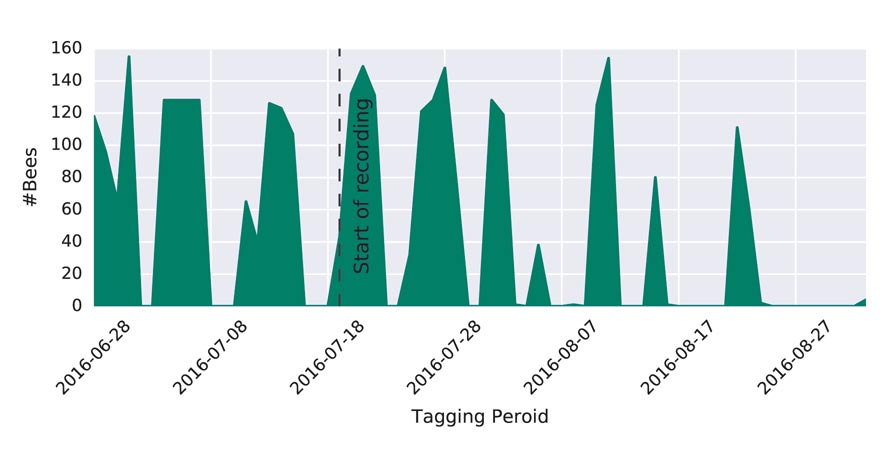
\includegraphics[width=1.0\textwidth]{Figures/tagging_period}
	\caption[Tagging Frequency]{Tagging frequency of bees: The bees were primarily tagged during the week. On average 48 bees were tagged each day, considering only tagging days, the average is about 91 ($\pm50$) bees (median 118).}
	\label{fig:tagging}
\end{figure}

The recording season lastet nine weeks (63 days), around the clock, from 19.07.2016 until 19.09.2016, with some interruptions due to maintainance and technical failures. I chose four consecutive days (30.07, 31.07, 1.8,2.8), marked in figure~\ref{fig:period} for further analysis and the 26.07. for testing purpose.

The recording resolution of each camera is three frames per second, with 1024 frames per video file. For each frame, bees were detected by using an image analysis pipeline, which is explained in detail in~\cite{wario2015automatic}. The resulting detection data is stored in a binary file format.
A python library called \emph{bb-binary}\footnote{\url{https://github.com/BioroboticsLab/bb_binary}; Last accesed: 2106-02-16, 04:28PM} provides easy access to the binary files. Each file in bb\_binary file format corresponds to a video file of a single camera.
The size of the complete dataset for 2016 is $470$~GB, about $7.5$~GB of binary data per day.

Exactly $3.191$ bees were tagged. The tagging period was 67 days long. The tagging started on 28.06.2016 (22 days before the recording started) and lasted until 02.09.2016 (17 days before the recording ended). The young bees were tagged and then added to the hive, about noon each day. The overall tagging frequency is shown in figure~\ref{fig:tagging}. The hatching day for each bee was documented. Therefore the age of each bee at a certain point in time can be calculated.

\subsection{Structure of the Dataset}
The data is organised in \emph{frame container}, wich corresponds to a video file of a single camera. A frame container holds all \emph{frames} for that specific video.
Each frame has a list of all detected bees.
A \emph{detection} has the following attributes, which are relevant to this project:

\begin{itemize}
\item \textbf{xpos}: $x$ coordinate of bee with respect to the image in pixel
\item \textbf{ypos}: $y$ coordinate of bee with respect to the image in pixel
\item \textbf{radius}: of the circular 12-bit tag
\item \textbf{decodedId}: decoded 12-bit id
\end{itemize}

Besides further information, the frame container specifies the camera, which took the video. A frame is also attributed with a timestamp. The data can be accessed iterating on the frame level, using two timestamps (start and end) for specifying the time interval. The complete data scheme can be found on github\footnote{\url{https://github.com/BioroboticsLab/bb_binary/blob/master/bb_binary/bb_binary_schema.capnp}; Last accessed: 2106-02-16, 04:46PM}. 


\subsection{ID Probabilities and Confidence Level}
\label{subsec:confidence}
With a 12-bit ID, 4096 bees can be tagged.
Each bit of the decodedId is not a $1$ or $0$, but represents a probability between $0$ and $255$. It indicates the reliablility of the image analysis pipeline for that specific bit.  A number closer to $255$ represents a $1$, a number closer to $0$ a $0$.
A \emph{confidence value} can be calculated for each ID. The confidence value of a single bit is its distance to $128$, discretized to a value between $0$ and $1$. The confidence value of an ID is therefore the minimum of all bit confidences. [TODO: in leons Arbeit ist das gut erklärt]

The amount of data that remains for further processing and its quality  depends heavily on the chosen \emph{confidence level}. Figure~\ref{fig:confidence} shows the relationship between confidence level, the amount of remainig data and the number of unique IDs. 

\begin{figure}
    \centering
    \begin{subfigure}[b]{0.45\textwidth}
        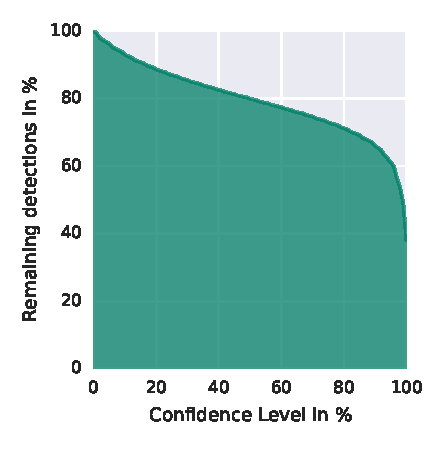
\includegraphics[width=\textwidth]{Figures/confVSamount}
        \caption[Remaining Detections]{Remaining Detections depending on the level of confidence.}
        \label{fig:confVSamount}
    \end{subfigure}
    \begin{subfigure}[b]{0.45\textwidth}
        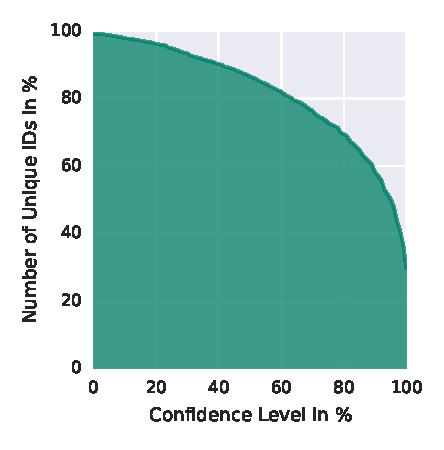
\includegraphics[width=\textwidth]{Figures/confVSids}
        \caption[Unique IDs]{Number of unique IDs depending on the level of confidence.}
        \label{fig:confVSids}
    \end{subfigure}

	\centering
	\begin{subfigure}[b]{0.45\textwidth}
		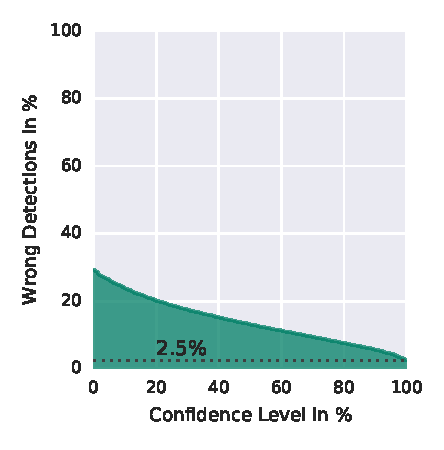
\includegraphics[width=\textwidth]{Figures/confVSdetquality}
		\caption[Wrong Detections]{Wrong detections in relation to the level of confidence.}
		\label{fig:confVSdetquality}
	\end{subfigure}
	\begin{subfigure}[b]{0.45\textwidth}
		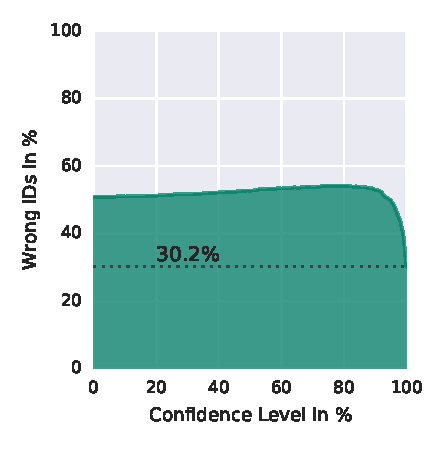
\includegraphics[width=\textwidth]{Figures/confVSidsquality}
		\caption[Unique IDs]{Number of wrong IDs depending on the level of confidence.}
		\label{fig:confVSidsquality}
	\end{subfigure}
	\caption[Data Quality]{The number of wrong detections decreases with an increasing level of confidence. In contrast, the number of false IDS becomes noticeably less only with a very high confidence level. The amount of remaining data decreases with an increasing confidence level. The number of unique IDs behave similar. (Dataset: 26.07.2016, 16:00-16:05) (Dataset: 26.07.2016, 16:00-16:05)}
	\label{fig:quality}
\end{figure}


\subsection{Time Series of Bees}
\label{subsec:tracking}

The original dataset (a number of frames containing bee detections), is transformed to binary \emph{time series of bees}, depicted in figure~\ref{fig:structure} (left and middle). A time series of a bee is a sequence of zeros and ones indicating the absence and presence of a bee over a specified time interval. 
As expected the confidence level has an effect on the resulting time series of a bee. A high confidence leads to more gaps in the series and also to more shorter gaps (see figure~\ref{fig:gaps}).

\begin{figure}[htb]
	\centering
	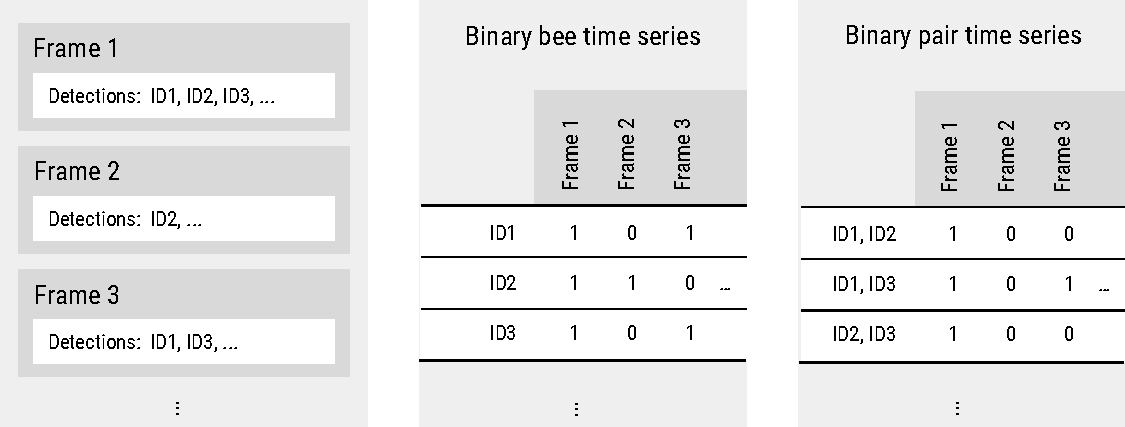
\includegraphics[width=1.0\textwidth]{Figures/structure}
	\caption[Structure of Dataset]{\textbf{Left:} original dataset - bb\_binary data containing frames and detections; \textbf{Middle:} transformation to time series - zero indicating absence of the bee, one indicating presence of the bee; \textbf{Right:} transformation to bee pairs - zero indicating eighter one or both bees are not present at the same time or not close to each other, one indicating bees are present at the same time and nearby.}
	\label{fig:structure}
\end{figure}

\begin{figure}
	\centering
	\begin{subfigure}[b]{0.45\textwidth}
		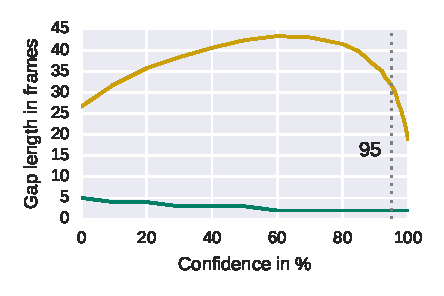
\includegraphics[width=\textwidth]{Figures/gaplen}
		\caption[Length of Gaps]{Length of Gaps depending on the level of confidence.}
		\label{fig:gaplen}
	\end{subfigure}
	\begin{subfigure}[b]{0.45\textwidth}
		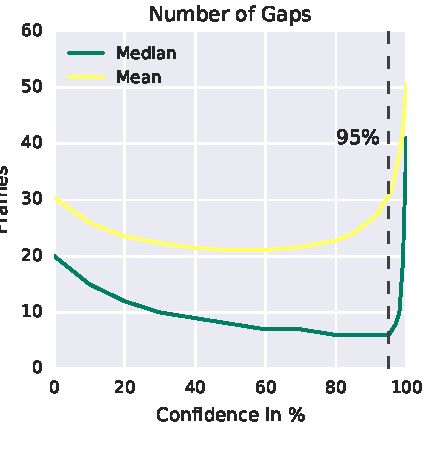
\includegraphics[width=\textwidth]{Figures/numgaps}
		\caption[Number of Gaps]{Number of Gaps depending on the level of confidence.}
		\label{fig:numgaps}
	\end{subfigure}
	\caption[Influence of Confidence Level on Gaps]{Influence of the confidence level of the length of gaps and number of gaps: With an increasing level of confidence the average gap length decreases and the number of gaps per bee series increases. (Dataset: 26.07.2016, 16:00-16:05)}
	\label{fig:gaps}
\end{figure}

\subsection{Data Quality}
\label{subsec:quality}

The quality of the data could be indirectly checked using the age information of bees. On 26.07.2016, about half of the bee tags ($2014$ of $4096$) were assigned to a bee. This day was chosen to determine the effects of the confidence level on data quality.
At first, for each detection the age of that bee was calculated, a negative age was counted as a wrong detection. I assumed that the number of wrong detections indicated by negative age also occured in the positive half, but remained unseen, therefore I doubled the error. Secondly, the number of wrong unique IDs is also determinde using the age test. Figure~\ref{fig:quality} shows that even though the number of wrong detections
decreases steadily with an increasing confidence level, but the number of wrong IDs only starts to decrease with a very high level.

Even with an confidence level of $100\%$, $30.2\%$ of the unique IDs are wrong (have a negative age), corresponding to only $2.5\%$ of detections. Therefore wrong IDs need to be filtered out anyway (independent of the confidence value), to obtain a more reliable dataset. A good indicator is the detection frequency of IDs. IDs with a negative age are on average less detected than IDs with a positive age.

\subsubsection{Frequency Filter}
IDs who definately exists, but their age can to be determinded are excluded from the analysis completely. These are bees, who were tagged later~($n=10$)\footnote{id= [2,
	74,
	2045,
	3172,
	3764,
	3796,
	3827,
	3836,
	3844,
	3940]} and IDs whos detection frequency is absurd high but there age is unknown~($n=7$)\footnote{id=[has changed! 
	17,
	168,
	801,
	888,
	2045,
	2357,
	2607]}

For each analysis day the number of detections per ID is obtained, excluding the mentioned IDs above. The frequency distribution tells that, IDs with a negative age are detected less often ($704$ frames $\pm 65$)  than bees with a positive age ($36.603$ frames $\pm 2.345$). The cutoff is 99\% of the negative IDs distribution. All IDs with a detection frequency below $4737 \pm 644$ frames are discarded. A list with possible (valid) IDs is kept for each day. Using this list, faulty detections can be filtered out beforehand.

\subsection{Implications}
For further analysis I use the following days: 14.08.2016, 17.08.2016, 20.08.2016, 02.09.2016 with a confidence level of $95\%$. This period is chose because of XY.

Because bee time series contain a lot of short gaps (mean = 3, 95\% confidence), the inferring of edges (bees who are close to each other at the same time), should be not that strict, or at least variable. This has to be taken into acoount, when looking at spatialy close bees.

\section{Inferring Networks}

The following part describes the pipeline for generating spatial proximity networks out of honey bee tracking data. A node in the network is a bee. They are distinguished by IDs. Only bees are in the network who interact at least once with another bee.

undirected and weighted, aggregated networks\\

Two bees are associated (spatially close to each other), if their distance is minor to a \emph{maximum distance}. As everything is very close in a bee hive this value is hard to choose. Only this criteria is very week, meaning having a resolution of three frames per seconds results in interactions which could only last for $0.33$ seconds. So an additional parameter the \emph{minimum contact duration} is introduced, it is the minimum time they have to spend at least nearby to be called associated.

Taking the fragmentation of tracks into account, it is obvious that two bees could be nearby but not at the very same time, but slightly shifted. So the minimum contact duration would be too errow prone. To overcome this issue one could correct the bee tracks, by filling gaps of varius sizes and interpolating the position of that bee accordingly. This is rather time consuming for this amount of tracking data (TODO: naja so doll auch nicht, scipy.ndimage.morphology.binary\_dilation) and also considering, that the tracking data is going to be improved in the future, then manipulating the raw data seems senseless. I rather perform a gap filling (maybe similar to binary dilation) on the time series of pairs, but not on the bee tracks, because this is independent of the input data.

Edges are attributed with two parameters. The first one is the frequency of contacts, so how often they share a close position. The second parameter is the total duration of contact, how many time frames in total they spend close by.

\subsection{Network Pipeline}

The network pipeline takes as input a path to the bb-binary data and outputs a graph in graphML file format. The pipeline takes the following parameters:

\begin{itemize}
\item path to data
\item confidence in percent
\item gap size in frames - this is used to corret the time series of bee pairs
\item maximum distance in px - define what close means (spatial proximity)
\item minimum contact duration in frames - how many frames bees need to spend nearby
\item cutoff in percent - IDs with a number of total detections below X percent of the mean frequency are discarded 
\item start timestamp - start of network slice
\item window size in minutes - size of time window for aggregating the network
\item number of used CPUs for parallelization
\item year - calculate IDs and set camera setup for 2015 or 2016
\end{itemize}

The pipeline is parallelized on frame level, that means, each process gets a portion (frames for a timeinterval of five minutes) of the data and extracts interactions/edges. The main process adds everything up and creates a network.
The steps are the following:

\begin{enumerate}
\item \textbf{Filter detections by confidence}\\
For each of the four camera the detections are filtered by the confidence level.

\item \textbf{Simple stitching}\\
Each side of the hive consists of two cameras. 	The $x$-coordinates of each detection (of the right	cameras) is moved further to the right, also adding an offset of $2\times \texttt{maximum distance}$. So the left and the right detection of each side of the hive are move into one reference system.

\item \textbf{Syncronize Cameras}\\
For each side of the hive the cameras need to be syncronized. In the normal case the difference between consecutive frames should be about $0.332$~seconds, due to technical problem this value can be lower ($0.003$ ) and higher ($2.932$) at certain times. Cameras 3 and 2 and cameras 1 and 0 are matched, frames without a match are dropped (shorter number of frames, matchen, threshold $0.33/2$, minimum).

\item \textbf{Discard Detections with certain IDs}\\
All detections whos ID is in a list are keept, other detections are discarded. (see frequency filter)

\item \textbf{Extract close pairs}\\
For each side of the hive, all close pairs according to the maximum distance parameter are calculated and then joined together.

\item \textbf{Generate time series of bee pairs}\\
The data structure (frames and detection) is transformed to time series of bee pairs.

\item \textbf{Correct pair time series.}\\
The time series of bees are corrected by filling in the gaps of length \texttt{gap size}.

\item \textbf{Extract edges}\\
The edges and its attributes (frequency and duration) are extracted from the time series of bees using the minimum contact duration parameter. A sequence of at least X ones counts as one interaction. The frequency of those series adn the total duration (number of ones) are the attributes.


\end{enumerate}

\subsection{Pipeline Parameters}
For performing the network analysis, I chose the pipeline parameters as follows:

\begin{description}
\item[Confidence] As explained in section\ref{subsec:confidence}, the confidence is set to $95\%$.

\item[Maximum Distance] I chose the length of a bee body, according to \textcite{baracchi2014socio}, as the maximum distance between two bees (figure~\ref{fig:radius}). The average bee length of $212$px ($\pm 16$px)  was determinded by manually measuring the length of all bees ($n=337$) in four images (one for each camera, 21.07.2016, 03:00PM) using the tool ImageJ\footnote{\url{http://imagej.net/Welcome}; Last accessed: 22.02.2016}.

\item[Gap Size] The gap size is set to two frames. This value corresponds to the median gap length in the time series of pairs ($\texttt{mode}=1$, $\texttt{mean}=27$). [TODO: what dataset was used (95\% confidence, XXX\% cutOff, XXXpx maximal distance, date, camera)]

\item[Minimum Contact Duration] This is set to three frames (one second). This corresponds to~\textcite{mersch2013tracking}, they as well exclude interactions below one second. Looking at the frequency distribution of chains of ones ($1$, $11$, $111$, and so on) of the pair time series (after filling the gaps), then: $\texttt{mode}=1$, $\texttt{median}=2$ and $\texttt{mean}=4$. Three frames corresponds to $57\%$ of all chains, this seem to be reasonable. [TODO: what dataset was used (95\% confidence, XXX\% cutOff, XXXpx maximal distance, date, camera)]

\end{description}

\begin{figure}[b]
	\centering
	\begin{subfigure}[b]{0.45\textwidth}
		\centering
		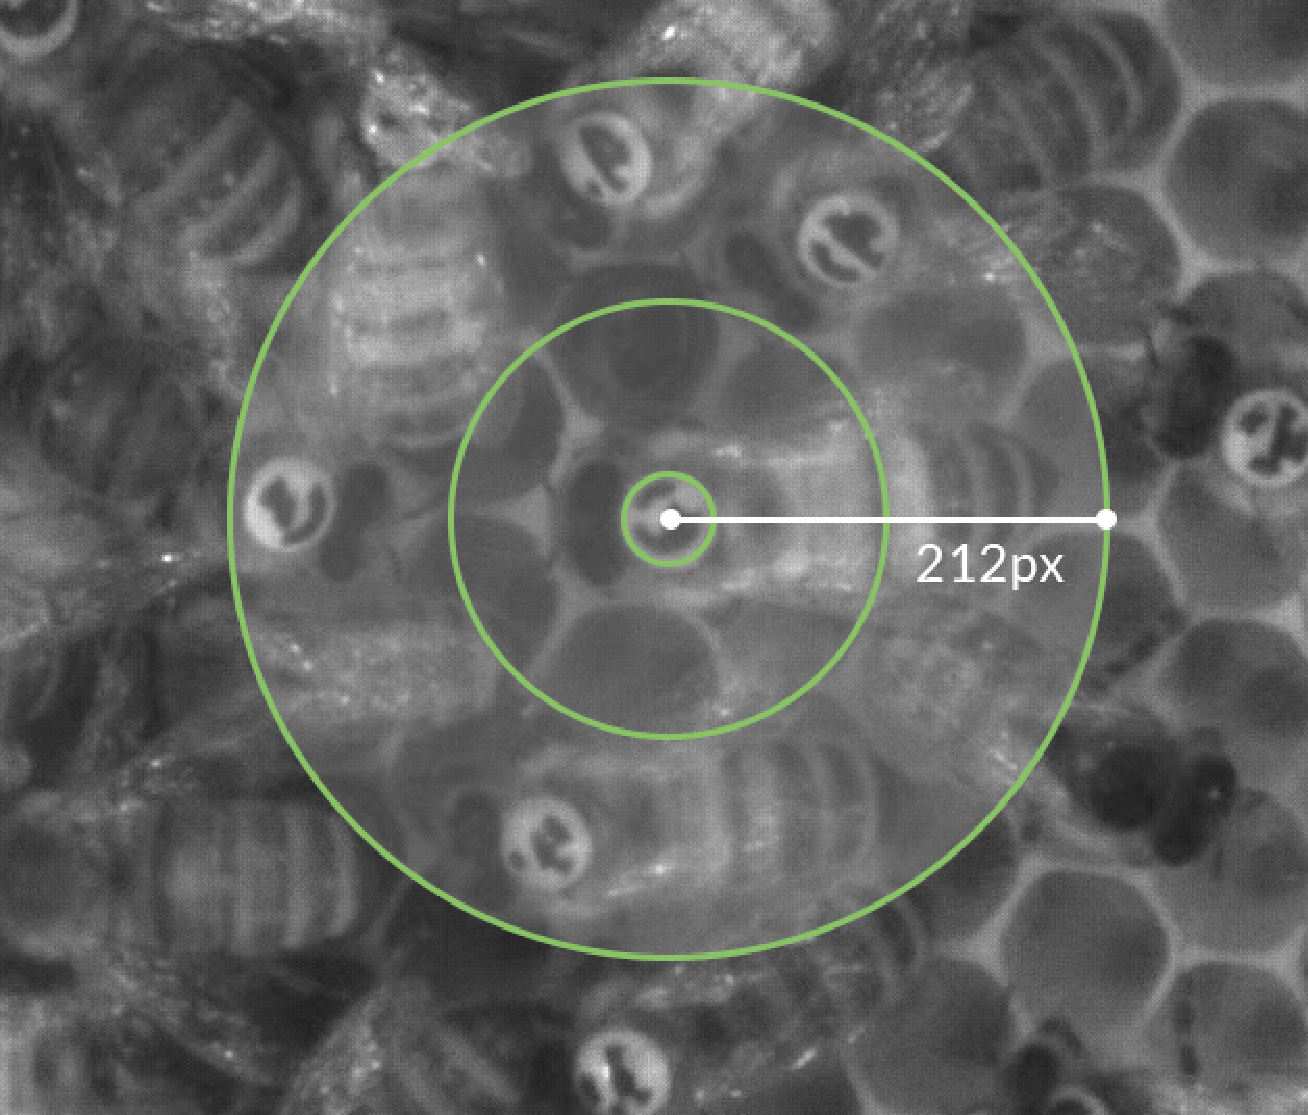
\includegraphics[width=\textwidth]{Figures/radius}
		\caption[Contact Radius]{Contact Radius}
		\label{fig:radius}
	\end{subfigure}
	~ %add desired spacing between images, e. g. ~, \quad, \qquad, \hfill etc. 
	%(or a blank line to force the subfigure onto a new line)
	\begin{subfigure}[b]{0.45\textwidth}
		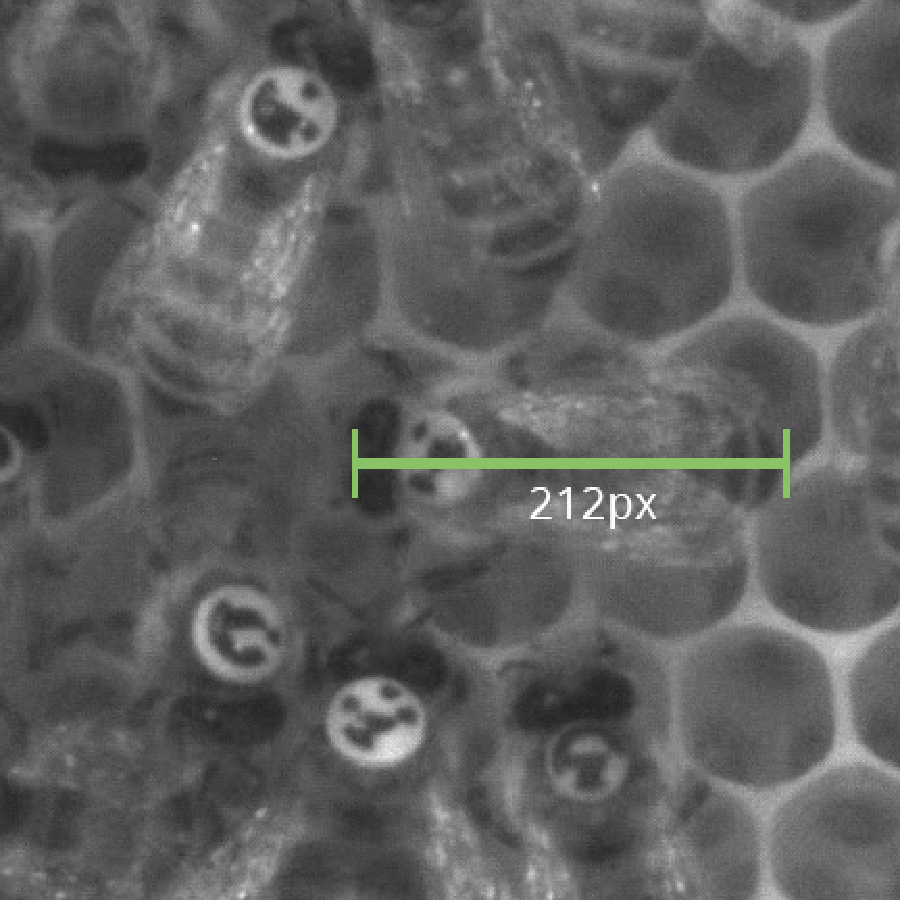
\includegraphics[width=\textwidth]{Figures/sizeTagBee}
		\caption[Bee and Tag Size]{Bee Length}
		\label{fig:size}
	\end{subfigure}
	\caption{Distance Between Bees: A length of a bee is chosen as the maximal  distance between bees.}
	\label{fig:contactRadius}
\end{figure}

The networks are not thresholded (according to~\cite{farine2015constructing}).

\section{Static and Temporal Analysis}

Despite the possibility of generating networks of different granularity (resolution is minutes), here for further analysis daily networks (10h, two hours after sunrise until zwo hours before sunset) are aggregated.

\subsection{Static Network Analysis}
The following network properties were analysed for a static day and hour network.\\
TODO: list of properties. (similar to what others have done)
nodes, edges, density, diameter\\


\subsection{Temporal Analysis}
three day networks (2 days gap)\\
one network 2 weeks later\\

\subsection{Community Detection}
I tested all community detection algorithms implemented in python, to find an algorithm, which works well for my case of animal social networks. The three most common python libraries for network analysis were reviewed: NetworkX\footnote{\url{https://networkx.github.io/}; Last accessed: 16.03.2016, 6:36~p.m.}, igraph\footnote{\url{http://igraph.org/python/}; Last accessed: 16.03.2016, 6:38~p.m.}, and graph-tool\footnote{\url{https://graph-tool.skewed.de/}; Last accessed: 16:03.2016, 6:39~p.m.})

The algorithm needs to fulfill the following criteria:

\begin{itemize}
\item Support for large and very dense networks ($N>1000$, $D>50~\%$)
\item Support weighted edges
\item Fast runtime
\item Detection of more than one community
\end{itemize}

Table~\ref{tab:algos} gives an overview about the twelve algorithms reviewed. Five algorithms did not terminate after 15~minutes and were therefore excluded from further investigations. The Louvain algorithm is the same as multilevel, but performs worse by a similar result (number and members of communities) and was also excluded. Walktrap was tested for different step size parameters as suggested in~\cite{pons2005computing}, the communities remained stable.

Finally, I chose the leading eigenvector community detection algorithm because~\cite{farine2015constructing} explain that this algorithm is often used with animal social networks and works well.

\begin{table}[htbp]
\small
\caption[Compairing community detection algorithms]{\textbf{Comparing community detection algorithms} Comparison of algorithms implemented in python. Criterias are the support of weighted edges, runtime and number of communities. A runtime indicated by $-$ mean no termination after 15~minutes.\\
}
\label{tab:algos}

\begin{tabularx}{\textwidth}{lcccccccccccc}
\toprule
	 {} &
	 \rotatebox{90}{\textbf{fastgreedy$^1$}} &
	 \rotatebox{90}{\textbf{leading eigenvector$^1$}} &
	 \rotatebox{90}{louvain$^2$} &
	 \rotatebox{90}{\textbf{multilevel$^1$}} &
	 \rotatebox{90}{\textbf{walktrap$^1$}} &
	 
	 \rotatebox{90}{infomap$^1$} &
	 \rotatebox{90}{label propagation$^1$} &
	 
	 \rotatebox{90}{edge betweenness$^1$} &
	 \rotatebox{90}{k-clique communities$^2$\thinspace} &
	 \rotatebox{90}{optimal modularity$^1$} &
	 \rotatebox{90}{spinglass$^1$} &
	 \rotatebox{90}{statistical inference$^3$} \\ \midrule
	 
	 
	 
	 Edge weights & $\times$ & $\times$ & $\times$ & $\times$ & $\times$ & $\times$ & $\times$ & & $\times$ & $\times$ & $\times$ \\ \midrule
	 Runtime in sec & ~$3.6$ & ~$6.3$ & $11.7$ & ~$0.7$ & $19.4$ & $13.2$ & ~$0.2$ & $-$ & $-$ & $-$ & $-$ & $-$ \\ \midrule
	 Communities & $3$ & $2$ & $2$ & $3$ & $2$ & $1$ & $1$ & $-$ & $-$ & $-$ & $-$ & $-$ \\ \midrule
	  & 473 & 488 & 469 & 462 & 490 & 922 &  922 &  &  &  &  &  \\
	  & 434 & 434 & 453 & 427 & 431 &  &  &  &  &  &  &  \\
	  & 15 &  &  & 33 & (1) &  &  &  &  &  &  &  \\
	 \bottomrule
	 
\end{tabularx}
\begin{flushright}
\footnotesize{
$^1$ igraph, $^2$ NetworkX, $^3$ graph-tool\\
}
\end{flushright}

\end{table}

% \hdashline
% \midrule
% \bottomrule


\section{Attributed Data and Hypothesis Testing}
Hypothesis\\
(1) Communities reflect groups of bees working in different areas of the hive and\\
(2) Communities reflect different age groups\\

The data which was used to test the hypothesis (1) is saved in a sqlite database for faster access, because using bb\_binary (parsing the data over and over again) was to slow. For testing if lists of positions (spatial ditribution) are different the test XY was used [TODO: what to use here]

For hypothesis (2) the data is stored as a csv file of birth dates of each bee. For testing if age goups are different the Kolmogorov Smirnov Test was used.

\section{Implementation, Runtime and Complexity}
For implementing the network pipeline python, with pandas and numpy, are used, because the bb\_binary library, for accessing the tracking, data is only available in python. The networks, in graphML format, are created using the python library \emph{NetworkX}\footnote{\url{https://networkx.github.io/} ; Last accessed: 2017-02-17, 08:07PM} in version 1.11.
iGraph for community detection\\
some bash scrips for generating multiple networks\\

bottleneck is reading bb\_binary data into pandas dataframes\\
using multithreading for distribution on frame level (a process gets X frames for processing)\\

maybe some table with how long nees what with how many cores (hom much RAM and so on)\\